\documentclass[hyperref, xcolor=dvipsnames, 10pt]{article} % use larger type; default would be 10pt
\usepackage[utf8]{inputenc} % set input encoding (not needed with XeLaTeX)
\usepackage{graphicx} % support the \includegraphics command and options
\usepackage{booktabs} % for much better looking tables
\usepackage{array} % for better arrays (eg matrices) in maths
\usepackage{paralist} % very flexible & customisable lists (eg. enumerate/itemize, etc.)
\usepackage{verbatim} % adds environment for commenting out blocks of text & for better verbatim
\usepackage{subfig} % make it possible to include more than one captioned figure/table in a single float
\usepackage{hyperref} % for urls
\usepackage{amsmath,amssymb,stmaryrd,mathtools}
\usepackage[framed]{matlab-prettifier}


\definecolor{lightgray}{gray}{0.5}
\definecolor{bggray}{gray}{0.95}
%\lstset{style=Matlab-editor,basicstyle=\scriptsize\mlttfamily, backgroundcolor=\color{bggray}}
\lstset{style=Matlab-editor,basicstyle=\footnotesize, backgroundcolor=\color{bggray}}

\usepackage{tikz}
\usetikzlibrary{positioning,arrows,chains,scopes,calc,fit,backgrounds}


%argmin
\DeclareMathOperator*{\argmin}{argmin}

% \renewcommand{\baselinestretch}{.9}

\def \r {\rho} 
\def \x {\mathbf{x}} 
\def \u {\mathbf{u}} 
\def \w {\mathbf{w}} 
\def \y {\mathbf{y}} 

\def \occ {\text{occ}}
\def \comf {\text{comf}}
\def \f {\varphi}

\def \refn {\text{ref}}
\def\dt{ \text{\small $\Delta$}t}

\def\X {{\cal X}}
\def\U {{\cal U}}
\def\W {{\cal W}}
\def\Y {{\cal Y}}

\def\wr {\w^{\text{ref}}}
\def\Reals {\mathbb{R}}


\def\G {\text{alw}} 
\def\F {\text{ev}} 
\def\until {\text{until}}

\newtheorem{problem}{Problem}


%\usepackage{titlesec}
%\titleformat{\section}{\large\bfseries}{\thesection}{1em}{}
%\renewcommand{\thefootnote}{\arabic{footnote}}

% ----------------------------------------------
\title{BluSTL: A Model Predictive Control Toolbox with Signal Temporal Logic Constraints}
\author{
Vasumathi Raman\footnote{United Technologies Research Center in Berkeley, CA}\hspace{1ex}
 and Alexandre Donz\'e\footnote{University of California, Berkeley}
}
% ----------------------------------------------
% Include a date to distinguish different versions.
% ----------------------------------------------
\date{v0.2, 2016-01-25 } 
% ----------------------------------------------

\begin{document}
\maketitle


\begin{abstract}
  We present BluSTL, a MATLAB toolbox for automatically generating controllers from
  specifications written in Signal Temporal Logic (STL). The toolbox takes as input a system and a
  set of constraints expressed in STL and constructs an open-loop or a closed-loop (in a receding
  horizon or Model Predictive fashion) controller that enforces these constraints on the system
  while minimizing some cost function. The controller can also be made reactive or robust to some
  external input or disturbances. The toolbox is available at \url{https://github.com/BluSTL/BluSTL}.
\end{abstract}

% ----------------------------------------------
\section{Introduction}
% ----------------------------------------------
In \cite{CDC14, HSCC15} we described a new technique for synthesizing controllers for hybrid systems
subject to specifications expressed in Signal Temporal Logic (STL). The present document introduces
the toolbox BluSTL, which implements the ideas presented in these papers. The toolbox takes as input
a linear system (which can result from the linearization of some non-linear system), a set
of constraints expressed in STL and a cost function and outputs a controller. The controller can be either in
\emph{open-loop}, i.e., it will compute a fixed sequence of inputs to be used by the system, or in
\emph{closed-loop} in a receding horizon fashion. In the latter case, a sequence of inputs is
computed at each step, and only the first input values is used for one time step, and the
process is reiterated. One specificity of the toolbox is that the user can tune the robustness of
satisfaction of the STL specifications as defined in \cite{DonzeM10}. The toolbox also supports
robust controller synthesis in more classical sense, i.e., robust to variations of some external
disturbance input.\\
 
The approach as described in \cite{CDC14,HSCC15} is based on encoding the system dynamics, the STL
constraints and the cost function together in a Mixed-Integer Linear Problem (MILP). The controller
then consists in a pre-compiled MILP which can be solved efficiently by modern MILP solvers, such as
Gurobi \cite{gurobi}. Experiments show that  the pre-compilation phase, which can be done
off-line, can take significantly more time (several seconds to minutes, depending on the complexity
of the dynamics and the specifications) than actually solving the resulting problem. The former can
be done often very quickly (less than a second), which makes it possible to use the resulting
controller on-line, possibly in real-time applications. The rest of the paper briefly describes the
theoretical background and then presents a small tutorial example.

% ----------------------------------------------
\section{Some Theoretical Background} 
% ----------------------------------------------

\subsection{System dynamics}
We consider a continuous-time system $\Sigma$ of the form 

\begin{eqnarray}
\dot{x} &= &A x + B_u u + B_w w \\ 
 y &=& C x + D_u u + D_w w
\end{eqnarray}
where 
\begin{itemize}
\item $x \in {\cal X} \subseteq \Reals^{n}$ is the \emph{system state},
\item $u \in \U \subseteq \Reals^{m}$ is the \emph{control input},
\item $w \in \W \subseteq \Reals^{l}$ is the \emph{external input}, 
\item $y \in \Y \subseteq \Reals^{o}$ is the \emph{system output}.
\end{itemize}

Given a sampling time $\dt>0$, we discretize $\Sigma$ into 
$\Sigma_d$ of the form
\begin{eqnarray}
x(t_{k+1}) &= &A^d x(t_k) + B^d_u u(t_k) + B^d_w w(t_k)  \label{eq:dynd} \\ 
 y(t_k) &=& C^d x(t_k) + D^d_u u(t_k) + D^d_w w(t_k)  \label{eq:outd}
\end{eqnarray}

where for all $k>0$, $t_{k+1}-t_k = \dt$ and $t_0=0$. Given an integer $N>0$, $x_0\in\X$, and two sequences 
$\u \in \U^{N-1}$ and $\w \in \W^{N-1}$ noted
\begin{eqnarray*}
\u&= u_0u_1\hdots u_{N-1}\\
\w&= w_0w_1\hdots w_{N-1}
\end{eqnarray*}
we denote by $\xi(x_0, \u, \w) \in \X^N$ the 4-uple of sequences
$(\x,\y,\u,\w) = \xi(x_0, \u, \w)$ such that $\x$, $\y$, $\u$ and $\w$ satisfy (\ref{eq:dynd}-\ref{eq:outd}) with
$x(t_k)=x_k$, $y(t_k)=y_k$, $u(t_k)=u_k$ and $w(t_k)=w_k$ for all $k$. $\xi(x_0, \u, \w)$, or
sometimes simply $\xi$ is called a run of $\Sigma_d$.

\def\Dxi{\X\times\Y\times\U\times\W}

\subsection{Signal Temporal Logic}
We consider STL formulas defined recursively according to the grammar\footnote{For the readers
  familiar with temporal logic, note that the notation $\F$ and $\G$ (for $\Box$ and $\Diamond$) are
  taken from the syntax also implemented in the toolbox Breach.}
$$
\f ::= \pi^\mu \mid \neg \psi \mid \f_1 \land \f_2 \mid \G_{[a,b]}~\psi \mid \f_1~\until_{[a,b]}~\f_2
$$

 where $\pi^\mu$ is an atomic predicate $\Dxi \rightarrow \mathbb{B}$ whose truth value is
determined by the sign of a function $\mu: \Dxi \rightarrow \Reals$ and $\psi$ is an STL
formula. The fact that a run $\xi(x_0, \u,\w)$ satisfies an STL formula $\f$ is denoted by
$\xi \models \f$. Informally, $\xi \models \G_{[a,b]} \f$ if
$\f$ holds at every time step between $a$ and $b$, and
$\xi \models \f~\until_{[a,b]}~\psi$ if $\f$ holds at every time step before $\psi$
holds, and $\psi$ holds at some time step between $a$ and $b$. Additionally, we define
$\F_{[a,b]}\f = \top~\until_{[a,b]}~\f$, so that $\xi \models \F_{[a,b]} \f$ if
$\f$ holds at some time step between $a$ and $b$. Formally, the validity of a formula $\f$ with
respect to the sequence $\x$ is defined inductively
as follows
\[
\begin{array}{lll}
\xi \models \f & \Leftrightarrow& (\xi,t_0) \models \f\\
(\xi,t_k) \models\pi^\mu &\Leftrightarrow& \mu(x_k,y_k,u_k,w_k) > 0\\
(\xi,t_k) \models \neg \psi &\Leftrightarrow& \neg((\xi,t_k) \models \psi)\\
(\xi,t_k) \models \f \land \psi &\Leftrightarrow& (\xi,t_k) \models \f \land (\xi,t_k) \models \psi\\
(\xi,t_k) \models \G_{[a,b]} \f &\Leftrightarrow& \forall t_{k'}\in [t_k\!+\!a, t_k\!+\!b], (\xi,t_{k'}) \models \f\\
 (\xi,t_k) \models \f~\until_{[a,b]}~\psi &\Leftrightarrow& \exists t_{k'} \in [t_k\!+\!a,t_k\!+\!b] \mbox{ s.t. } (\xi,t_{k'}) \models \psi \\
&&\land \forall t_{k''} \in [t_{k},t_{k'}], (\xi,t_{k''}) \models \f.
\end{array}
\]
An STL formula $\f$ is \emph{bounded-time} if it contains no unbounded operators; the
\emph{bound} of $\f$ is the maximum over the sums of all nested upper bounds on the temporal
operators, and provides a conservative maximum trajectory length required to decide its
satisfiability. For example, for $\G_{[0,10]} \F_{[1,6]} \f$, a trajectory of length
$N \ge 10 + 6 = 16$ is sufficient to determine whether the formula is satisfiable. 

\subsection{Robust Satisfaction of STL formulas}\label{robust_defn}

Quantitative or robust semantics defines a real-valued function $\r^\f$ of signal $\xi$ and $t$ such
that $(\xi,t) \models \f \equiv \r^\f(\xi,t) > 0$. In this work, it is defined as follows:
\[
\begin{array}{lll}
\r^{\pi^\mu}(\xi,t_k)&=& \mu(x_k,y_k,u_k,w_k)\\
\r^{\neg \psi}(\xi,t_k)&=&  -\r^\psi(\xi, t_k) \\
\r^{\f_1 \land \f_2}(\xi,t_k)&=& \min (\r^{\f_1}(\xi,t_k),\r^{\f_2}(\xi,t_k)    )\\
\r^{\f_1 \lor \f_2}(\xi,t_k)&=& \max (\r^{\f_1}(\xi,t_k),\r^{\f_2}(\xi,t_k)    )\\
\r^{\G_{[a,b]} \psi}(\xi,t_k)&=& \min_{t_{k'}\in [t+a, t+b]}\r^{\psi}(\xi,t_{k'})\\
\r^{\f_1~\until_{[a,b]}~\f_2}(\xi,t_k)&=&  \max_{t_{k'}\in [t+a, t+b]} ( \min (\r^{\f_2}(\xi,t_{k'}),    \\
&&~~~~~~~~~~~~~~\min_{t_{k''} \in [t_k,t_{k'}]} \r^{\f_1}(\xi,t_{k''}))
\end{array}
\]

To simplify notation, we denote $\r^{\pi^\mu}$ by $\r^{\mu}$ for the remainder of this document. The
robustness of satisfaction for an arbitrary STL formula is computed recursively from the above
semantics by propagating the values of the functions associated with
each operand using $\min$ and $\max$ operators corresponding to the various STL operators. For
example, the robust satisfaction of $\pi^{\mu_1}$ where $\mu_1(x) = x-3>0$ at time $0$ is
$\r^{\mu_1}(\xi,0) = x_0-3$. The robust satisfaction of $\mu_1 \wedge \mu_2$ is the minimum of
$\r^{\mu_1}$ and $\r^{\mu_2}$. Temporal operators are treated as conjunctions and disjunctions along
the time axis: since we deal with discrete time, the robustness of satisfaction of
$\f= \G_{[0,2.1]} \mu_1$ is
$$\r^\f(x,t)= \min_{t_k \in [0,2.1]} \r^{\mu_1}(x,t_k)= \min \{x_0-3, x_1-3, \hdots, x_K-3\}$$ 
  where  $0 \leq t_0 < t_1 < \hdots < t_K \leq 2.1 < t_{K+1} $.

  The robustness score $\r^\f(\xi,t)$ should be interpreted as \emph{how much} $\xi$ satisfies
  $\f$. Its absolute value can be viewed as the signed distance of $\xi$ from the set of trajectories
  satisfying or violating $\f$, in the space of projections with respect to the function $\mu$ that
  define the predicates of $\f$ (\cite{FainekosP09}).

\subsection{Controller Synthesis}

Given an STL formula $\f$ and a \emph{cost function} of the form $J(x_0,\u,\w,\f) \in \Reals$,
BluSTL can solve different control synthesis problem, either in \emph{open loop} or \emph{closed
  loop}, and with a \emph{deterministic} or \emph{adversarial} environment (robust control). In all
problems, we assume given an initial state $x_0 \in \X$, an horizon $L$ and some reference
disturbance signal $\w \in \W^N$. The open loop and closed loop scenario are depicted as block
diagrams on Figure~\ref{fig:open} and Figure~\ref{fig:closed}.

\begin{problem}[Open loop, deterministic]\label{prob:open}
Compute $\u^*=u_0^*u_1^*\hdots u_{N-1}^*$ where
$$
\begin{array}{lll}
\u^*=& \displaystyle \argmin_{\u \in \U^N} J(x_0, \u, \w, \f)\\
&\mbox{s.t. } \xi(x_0, \u, \w) \models \varphi
\end{array}
$$
\end{problem}

Note that we assume that the state of the plant is fully observable.

\begin{figure}[h]
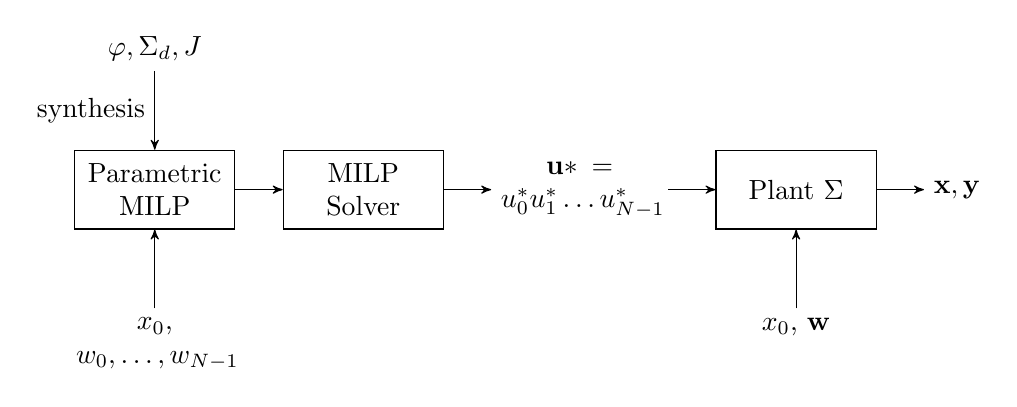
\begin{tikzpicture}[node distance=.6cm, >=stealth',every join/.style=->,
box/.style={draw, text centered, text width=1.8cm, minimum height=1cm},
nobox/.style={text centered, text width=2cm}
]
  
\node (in) [nobox] {$\f,\Sigma_d,J$};
\node (milp) [box, below=1cm of in] {Parametric MILP};
\node (solver) [box, right=of milp] {MILP Solver};
\node (sol) [nobox,right=of solver] {$\u*=$ $u^*_0u^*_1\hdots u^*_{N-1}$};
\node (plant) [box, right= of sol] {Plant $\Sigma$};
\node (trace) [right= of plant] {$\x,\y$};  
\node (x0wd) [nobox, below= 1cm of milp] {$x_0$, $w_0,\hdots,w_{N-1}$};
\node (x0w) [nobox, below= 1cm of plant] {$x_0$, $\w$};


\draw[->] (in) -- node [left] {synthesis} (milp);
\draw[->] (x0wd) -- (milp);  
\draw[->] (x0w) -- (plant);  

{[start chain]
\chainin (milp) [join];
\chainin (solver) [join];
\chainin (sol) [join];
\chainin (plant) [join];
\chainin (trace) [join];

}

\end{tikzpicture}
\caption{Open Loop Scenario. A parametric Mixed-Integer Linear Program is generated from the STL
  formula $\phi$, the discrete-time plant model $\Sigma_d$ and the cost function $J$. The parameters
of this MILP are the initial state $x_0$ and disturbance vector $\w$. When those are provided, a
solver can compute an optimal solution $\u^*$ for horizon $N$ which is passed and used by the
plant $\Sigma$.}  
\label{fig:open}
\end{figure}


\begin{problem}[closed loop, deterministic]\label{prob:det}
Given an horizon $0<L<N$, for all $0 \leq k \leq N-L$, compute $u_k^*$ as the first element of the
sequence $\u_k^L*=u_k^L*u_{k+1}^L*\hdots u_{k+L-1}^L*$ satisfying 
$$
\begin{array}{lll}
\u_k^L*=& \displaystyle \argmin_{\u^L_K \in \U^L} J(x_k, \u_k^L, \w_k, \f)\\
&\mbox{s.t. } \xi(x_k, \u^L_k, \w_k) \models \varphi
\end{array}
$$
\end{problem}

\begin{figure}[h]


  \begin{center}
    
 
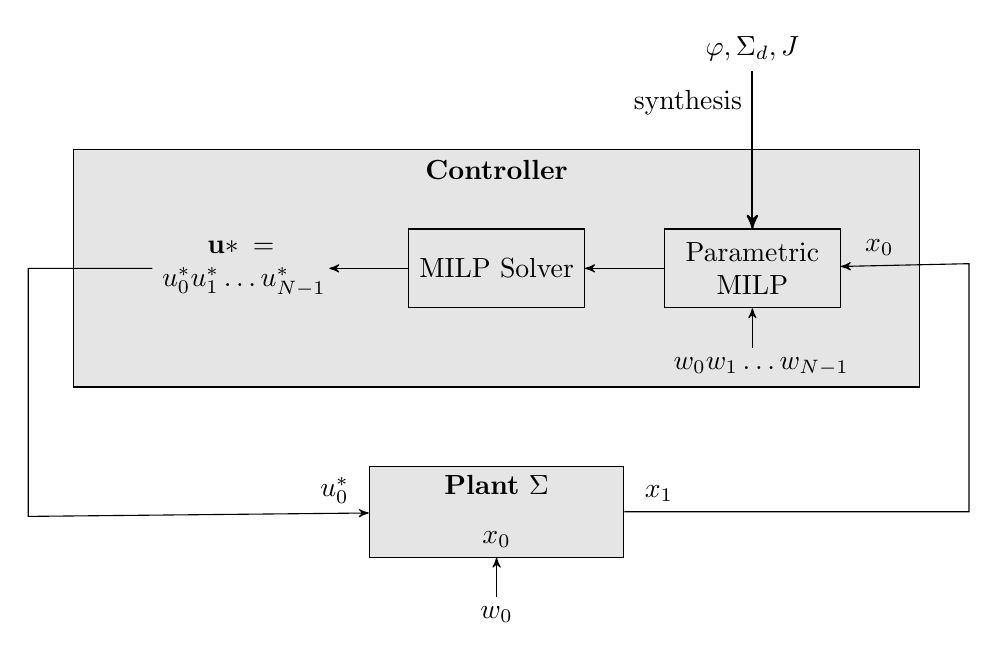
\begin{tikzpicture}[node distance=1 cm, >=stealth',every join/.style=->,
box/.style={draw, text centered, text width=2cm, minimum height=1cm},
nobox/.style={text centered, text width=2cm}
]

\node (sol) [nobox] {$\u*=$ $u^*_0u^*_1\hdots u^*_{N-1}$};
\node (solver) [box, right=of sol] {MILP Solver};
\node (milp) [box, right= of solver] {Parametric MILP};
\node (in) [nobox, above=2cm of milp] {$\f,\Sigma_d,J$};
\node (controller) [above=.5cm of solver] {\bf Controller}; 

\node (plant) [box, below= 2cm of solver, fill=black!10, text width=3cm] {\textbf{Plant $\Sigma$}\\[.2cm]  $x_0$};
\node (w0p) [nobox, below= .5cm of plant] {$w_0$};
\node (w0d) [nobox, below= .5cm of milp] {$w_0w_1\hdots w_{N-1}$};


\begin{pgfonlayer}{background}
    \node [draw, inner sep = 1cm, minimum height=1.8cm, fill=black!10,fit=(milp) (solver) (sol)] {};
  \end{pgfonlayer}

\draw[->, thick] (in) -- node [pos=0.2,left] {synthesis} (milp);
\draw[->] (w0d) -- (milp);  
\draw[->] (w0p) -- (plant);  

{[start chain]
\chainin (milp) [join];
\chainin (solver) [join];
\chainin (sol) [join];
}

\draw[->] (sol) -- ++(-2.7,0) -- ++(0,-3.15) -- (plant) node [pos=0.9, above] {$u_0^*$};
\draw[->] (plant) -- ++(6,0) node [pos=0.1, above] {$x_1$} -- ++(0,3.15) -- (milp) node [pos=0.7, above] {$x_0$};


\end{tikzpicture}
 \end{center}

\caption{Closed-loop Scenario. As for the open loop scenario, a parametric MILP is synthesized from
  the specifications, dynamics and cost function. However, at each time step, only the first optimal
input is used by the plant.}  
\label{fig:closed}
\end{figure}


These two problems both admit an adversarial version where $\w$ is allowed to vary in some region
around $\wr$ while satisfying some constraints. In this case, BluSTL treats $\w$ as an adversary
for the controller which tries to falsify $\f$. The control input returned by BluSTL, if any, is the
first one after some iterations for which this falsification is infeasible. If no such input is
found, BluSTL stops and declares the problem infeasible. We refer the reader to \cite{HSCC15} for more
details. 

%
% ----------------------------------------------
\section{Getting Started}
% ----------------------------------------------
%
\subsection{Installing BluSTL}
BluSTL depends on YALMIP \cite{YALMIP}, which is best obtained with the Multi-Parametric toolbox
(MPT3) \cite{MPT3}. Most experiments have been done with the Gurobi solver \cite{gurobi} as
back-end, though other solvers might work as well. Once YALMIP (or MPT3) is installed, the only thing to do to
install BluSTL is to add the path \verb+BluSTL/src+ to Matlab paths. In the following, we present a
tutorial example for a simple double integrator system. The tutorial script can be found in \verb+BluSTL/examples/tutorial1.m+.

%
% ----------------------------------------------
\section{Tutorial}
% ----------------------------------------------
% 

\input{tutorial1.tex}


%
% ----------------------------------------------
\section{Future Work}
% ----------------------------------------------
%
BluSTL v0.1 is still at an early stage of development, and beside the usual bug fixes,
performance and stability issues, it can be further improved in many directions. One limitation is
that unbounded specifications are currently limited to $\G (\f)$ where $\f$ is a bounded horizon
formula, where the horizon should be smaller than $L\times ts$. We are working on supporting more
unbounded horizon specifications, including $\F$ and $\until$ with possible nesting (e.g. $\F\ \G$
or $\G\ \F$). Another direction is to lift the constraint on the horizon of sub-formulas, by using
other semantics, e.g., \emph{weak} semantics, adapted to partial traces. Another limitation is on
the type of systems considered. It is relatively easy to use BluSTL for any kind of systems that
admit a proper linearization, but the linear models used in BluSTL are fixed. It would be
interesting to implement controller with switched linear dynamics, or more general hybrid models
such as, e.g., Mixed Logical Dynamics used in the MPT.  



\bibliographystyle{abbrv}
\bibliography{BluSTL_bib}

%
\end{document}
